%----------------------------------------------------------------------------------------
%	PACKAGES AND OTHER DOCUMENT CONFIGURATIONS
%----------------------------------------------------------------------------------------

\documentclass[paper=a4, fontsize=11pt]{scrartcl} % A4 paper and 11pt font size

\usepackage[T1]{fontenc} % Use 8-bit encoding that has 256 glyphs
\usepackage{fourier} % Use the Adobe Utopia font for the document - comment this line to return to the LaTeX default
\usepackage[english]{babel} % English language/hyphenation
\usepackage{amsmath,amsfonts,amsthm, amssymb} % Math packages
\usepackage[utf8]{inputenc}

\usepackage{graphicx}
\usepackage{float}

\usepackage{lipsum} % Used for inserting dummy 'Lorem ipsum' text into the template

\usepackage{sectsty} % Allows customizing section commands
\allsectionsfont{\centering \normalfont\scshape} % Make all sections centered, the default font and small caps

\usepackage{fancyhdr} % Custom headers and footers
\pagestyle{fancyplain} % Makes all pages in the document conform to the custom headers and footers
\fancyhead{} % No page header - if you want one, create it in the same way as the footers below
\fancyfoot[L]{} % Empty left footer
\fancyfoot[C]{} % Empty center footer
\fancyfoot[R]{\thepage} % Page numbering for right footer
\renewcommand{\headrulewidth}{0pt} % Remove header underlines
\renewcommand{\footrulewidth}{0pt} % Remove footer underlines
\setlength{\headheight}{13.6pt} % Customize the height of the header

\numberwithin{equation}{section} % Number equations within sections (i.e. 1.1, 1.2, 2.1, 2.2 instead of 1, 2, 3, 4)
\numberwithin{figure}{section} % Number figures within sections (i.e. 1.1, 1.2, 2.1, 2.2 instead of 1, 2, 3, 4)
\numberwithin{table}{section} % Number tables within sections (i.e. 1.1, 1.2, 2.1, 2.2 instead of 1, 2, 3, 4)

\setlength\parindent{0pt} % Removes all indentation from paragraphs - comment this line for an assignment with lots of text

%----------------------------------------------------------------------------------------
%	TITLE SECTION
%----------------------------------------------------------------------------------------

\newcommand{\horrule}[1]{\rule{\linewidth}{#1}} % Create horizontal rule command with 1 argument of height

\title{	
    \normalfont \normalsize 
    \textsc{TDT4173 - Machine Learning \& Case-based Reasoning, IDI, NTNU} \\ [25pt] % Your university, school and/or department name(s)
    \horrule{0.5pt} \\[0.4cm] % Thin top horizontal rule
    \huge Problem set 4 - Theory \\ % The assignment title
    \horrule{2pt} \\[0.5cm] % Thick bottom horizontal rule
}

\author{Øyvind Robertsen} % Your name

\date{\normalsize\today} % Today's date or a custom date

\begin{document}

\maketitle % Print the title

%----------------------------------------------------------------------------------------
%	PROBLEM 1
%----------------------------------------------------------------------------------------

\section{Theory}

\subsection{Basic Concepts}

\subsubsection{Well-posed learning problems}

A well-posed learning problem is a problem for which we can develop a program processing experience $E$ with respect to some class of tasks $T$ and performance measure $P$, to solve the problem. The program is said to \textbf{learn} if its performance at tasks in $T$, as measured by $P$, improves with experience $E$. \\

Examples of relevant machine-learning problems:

\begin{description}
    \item \textbf{Facial recognition} \hfill \\
        \begin{itemize}
            \item \textbf{Task T:} Recognizing faces in and across images.
            \item \textbf{Performance measure P:} Percentage of faces correctly reco gnized.
            \item \textbf{Training experience E:} Database of images with faces correctly classified.
        \end{itemize}
    \item \textbf{Sentiment analysis} \hfill \\
        \begin{itemize}
            \item \textbf{Task T:} Correctly recognize sentiment in natural language.
            \item \textbf{Performance measure P:} Degree of correctness as judged by a human supervisor.
            \item \textbf{Training experience E:} Corpus of natural language text with correct classifications.
        \end{itemize}
\end{description}

\subsubsection{Inductive bias}

Inductive bias refers to the set of assumptions a learning algorithm uses to produce output for input it has not previously encountered.
The goal of machine learning methods is to extrapolate and learn general concepts from subsets of large spaces (i.e. a hypothesis space).
If a machine learning algorithm bases itself on an unfit inductive bias, its ability to do exactly this will be limited. \\

In the candidate elimination algorithm, we assume that the target concept $c$ is contained in the initial hypothesis space $H$.

The ID3 algorithm is biased towards shorter trees with high information gain attributes close to the root.

\subsubsection{Overfitting}

Overfitting in machine learning refers to the case where a learning algorithm is more accurate in fitting known data than it is at predicting new data.
Biases that allow a learner to learn anything can result in overfitting.
Patterns in random data that is actually unrelated to the desired target function, will also be picked up by the learner.

\subsection{Candidate Elimination}

\subsubsection{Training and classification}

Sets $S$ and $G$ throughout training:

\begin{gather*}
    S_0 = \{<\varnothing, \varnothing, \varnothing, \varnothing, \varnothing>\} \\
    G_0 = \{<?, ?, ?, ?, ?>\}
\end{gather*}

\begin{gather*}
    S_1 = \{<hair, live, false, false, flat>\} \\
    G_1 = \{<?, ?, ?, ?, ?>\}
\end{gather*}

\begin{gather*}
    S_2 = \{<hair, live, false, false, flat>\} \\
    G_2 = \{<hair, ?, ?, ?, ?>, <?, live, ?, ?, ?>, <?, ?, false, ?, ?>, <?, ?, ?, false, ?>, <?, ?, ?, ?, flat>\}
\end{gather*}

\begin{gather*}
    S_3 = \{<hair, live, false, false, ?>\} \\
    G_3 = \{<hair, ?, ?, ?, ?>, <?, live, ?, ?, ?>, <?, ?, false, ?, ?>, <?, ?, ?, false, ?>\}
\end{gather*}

Classifying example 1:

\begin{gather*}
    <hair, live, false, false, none> \vdash true
\end{gather*}

Classifying example 2:

\begin{gather*}
    <feathers, egg, false, true, pointed> \vdash ?
\end{gather*}

Classifying example 3:

\begin{gather*}
    <scales, egg, true, false, flat> \vdash ?
\end{gather*}

\subsubsection{Remarks}

The last two examples can not be classified because they contain attribute values not encountered during training.
Further training on relevant examples would be necessary to classify these.
The first example conforms perfectly to training data, so it is successfully classified.

\subsubsection{Further training}

We want training data that further narrows the hypothesis space.
Either of the last two classification test examples would be good for training.

\section{Programming}

\subsection{Initial parameters}

The initial parameters were as follows:

\begin{gather*}
    W = [0.5, 0.5] \qquad b = 0 \qquad \alpha = 0.5 
\end{gather*}

These parameters were chosen by intuition and experimentation.
For instance, by looking at the datasets, we see that all input/output values are in the $[0, 1]$ range.
Using $[0, 0]$ as a weight vector would yield too low results, while $[1, 1]$ too high.
The middle of the two was concequently chosen.
Similar reasoning was used to choose the initial bias.

The learning rate was chosen through experimentation.

\subsection{Results and discussion}

Figure \ref{fig:loss-change} shows how the value of the loss function $L$ changed during training.
The 5th and 10th iteration are shown with dashed, red lines.

The 5th iteration had the following values:

\begin{gather*}
    W = [0.49210, 0.52288] \qquad b = 0.01711 \qquad L = 0.00831
\end{gather*}

Similarily, for the 10th iteration:

\begin{gather*}
    W = [0.47713, 0.52873] \qquad b = 0.02196 \qquad L = 0.00820
\end{gather*}

The final results:

\begin{gather*}
    W = [0.40221, 0.55595] \qquad b = 0.04727 \qquad L = 0.00796
\end{gather*}


\begin{figure}[H]
    \centering
    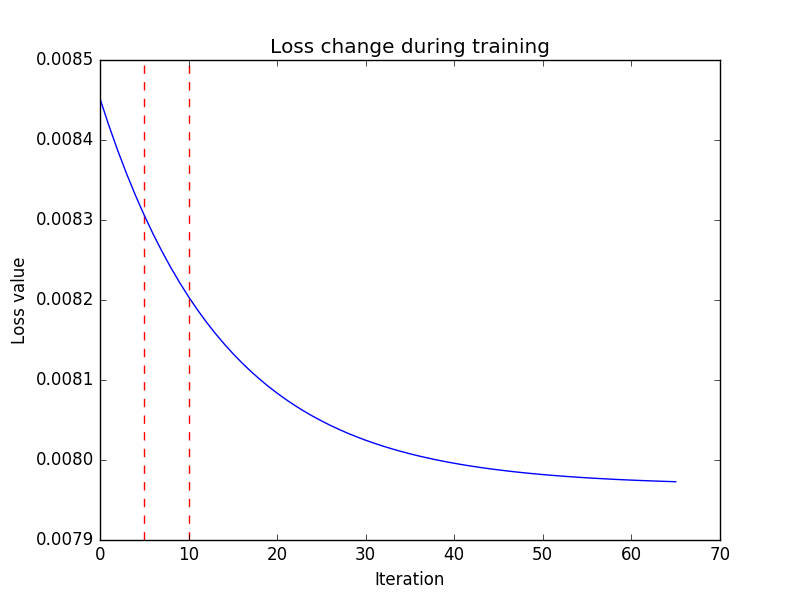
\includegraphics[width=0.8\linewidth]{img/loss-change.png}
    \caption{Change in loss during training} \label{fig:loss-change}
\end{figure}

\end{document}

